
\subsection{地表水额度分配与水需求的不匹配}

\begin{figure}[htb]
    \centering
    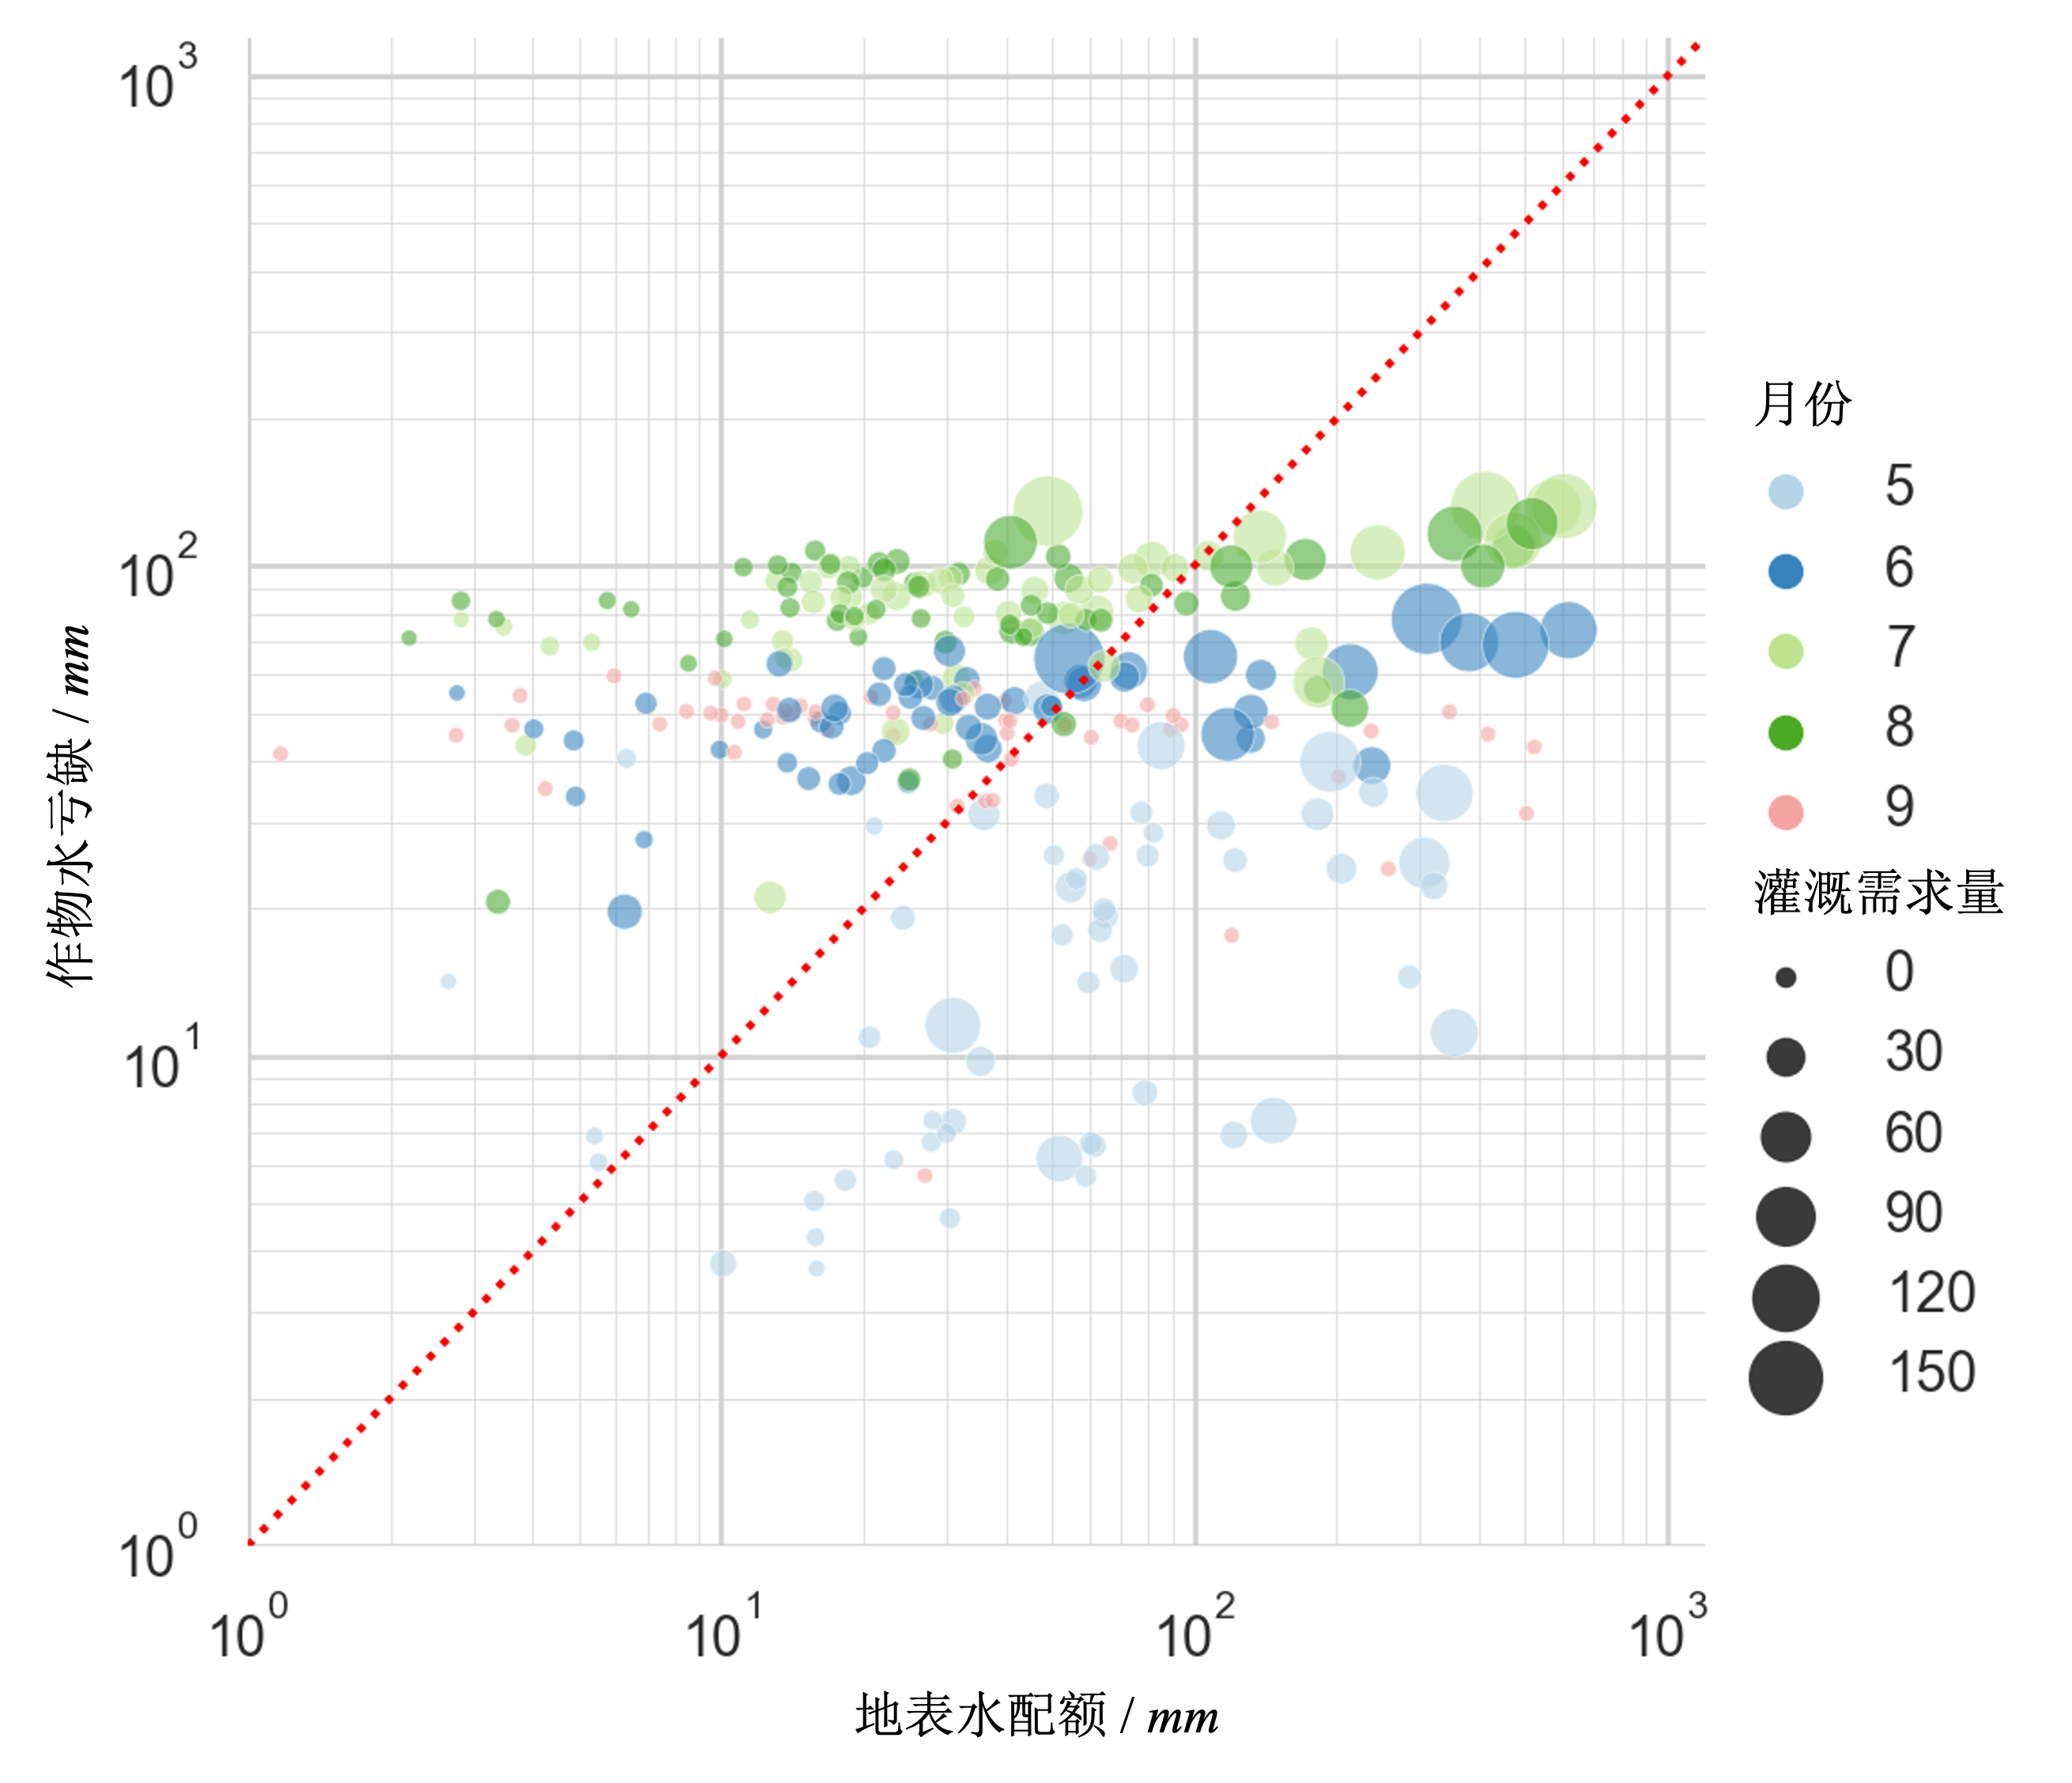
\includegraphics[width=\textwidth]{img/ch6/ch6_matches.png}
    \caption{各地级市月用水额度与用水需求的匹配情况}\label{ch6:fig:matches}
\end{figure}

\subsection{用水者决策对分水制度变化的响应}

由于社会系统存在决策行为的学习传播过程,违背制度进行超额取水的主体比例会随模拟时间而变化且存在阈值效应

配额如果不能满足大多数主体需求,违背制度的决策就会胜出,如青海、内蒙、河南、山东都偏向于违背分水配额,这与第五章识别的超额取水模式大体一致

\begin{figure}[htb]
    \centering
    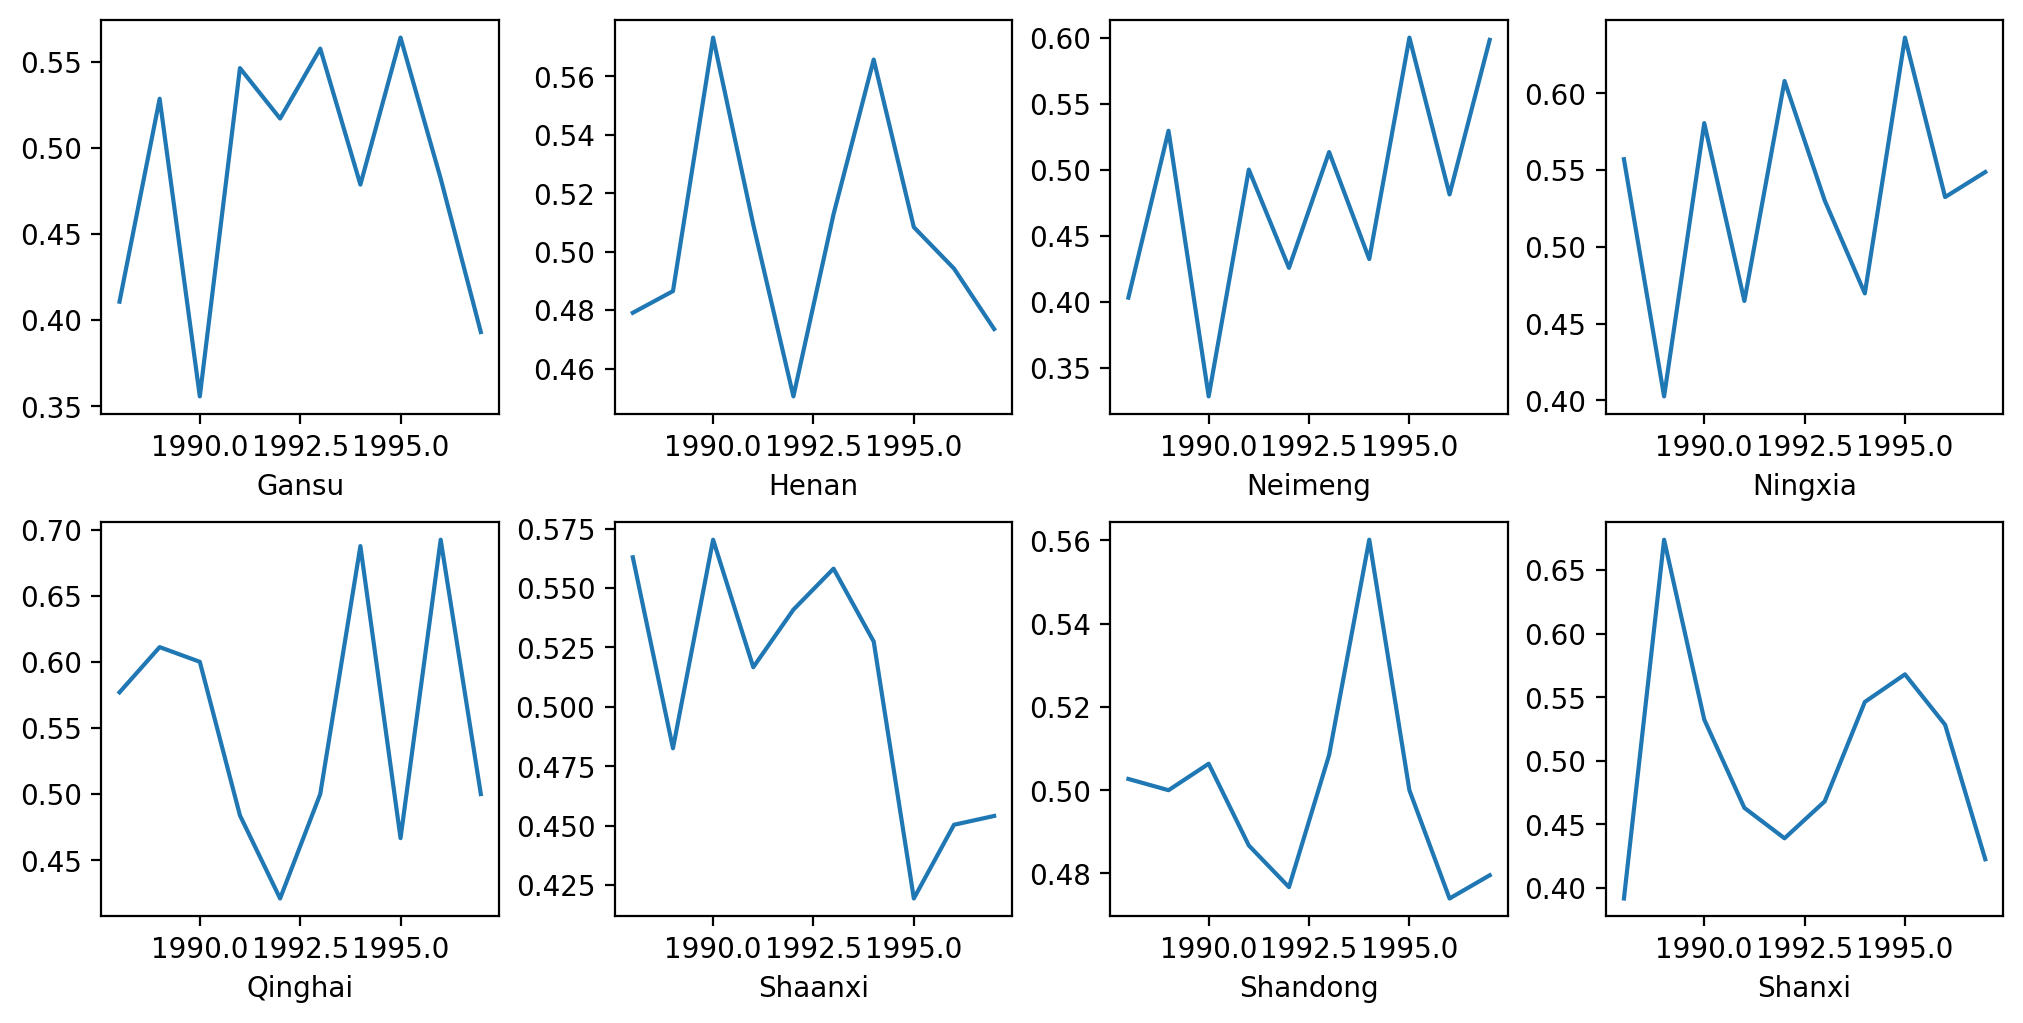
\includegraphics[width=\textwidth]{img/ch6/ch6_threshold.png}
    \caption{改变配额制度}\label{fig:xfig0}
\end{figure}

\subsection{用水来源对分水制度变化对的响应}

黄河流域作物生长的主要水源是绿水。研究表明,各省在总体上保持了蓝水使用占比持续下降的趋势,但是对用蓝/绿水比例的影响并不明显,仅有个别省份存在突变。
因此,为了更好地保护黄河流域的水资源,需要对各省的蓝水和绿水的使用情况进行深入研究,以便更好地理解不同省份之间的差异和变化。
此外,还需要进一步探讨各省份之间绿水资源的分配情况,以及如何更好地利用绿水资源来支持作物的生长和发展。这些研究结果对于制定更好的水资源管理政策和措施具有重要的意义。

\begin{figure}[htb]
    \centering
    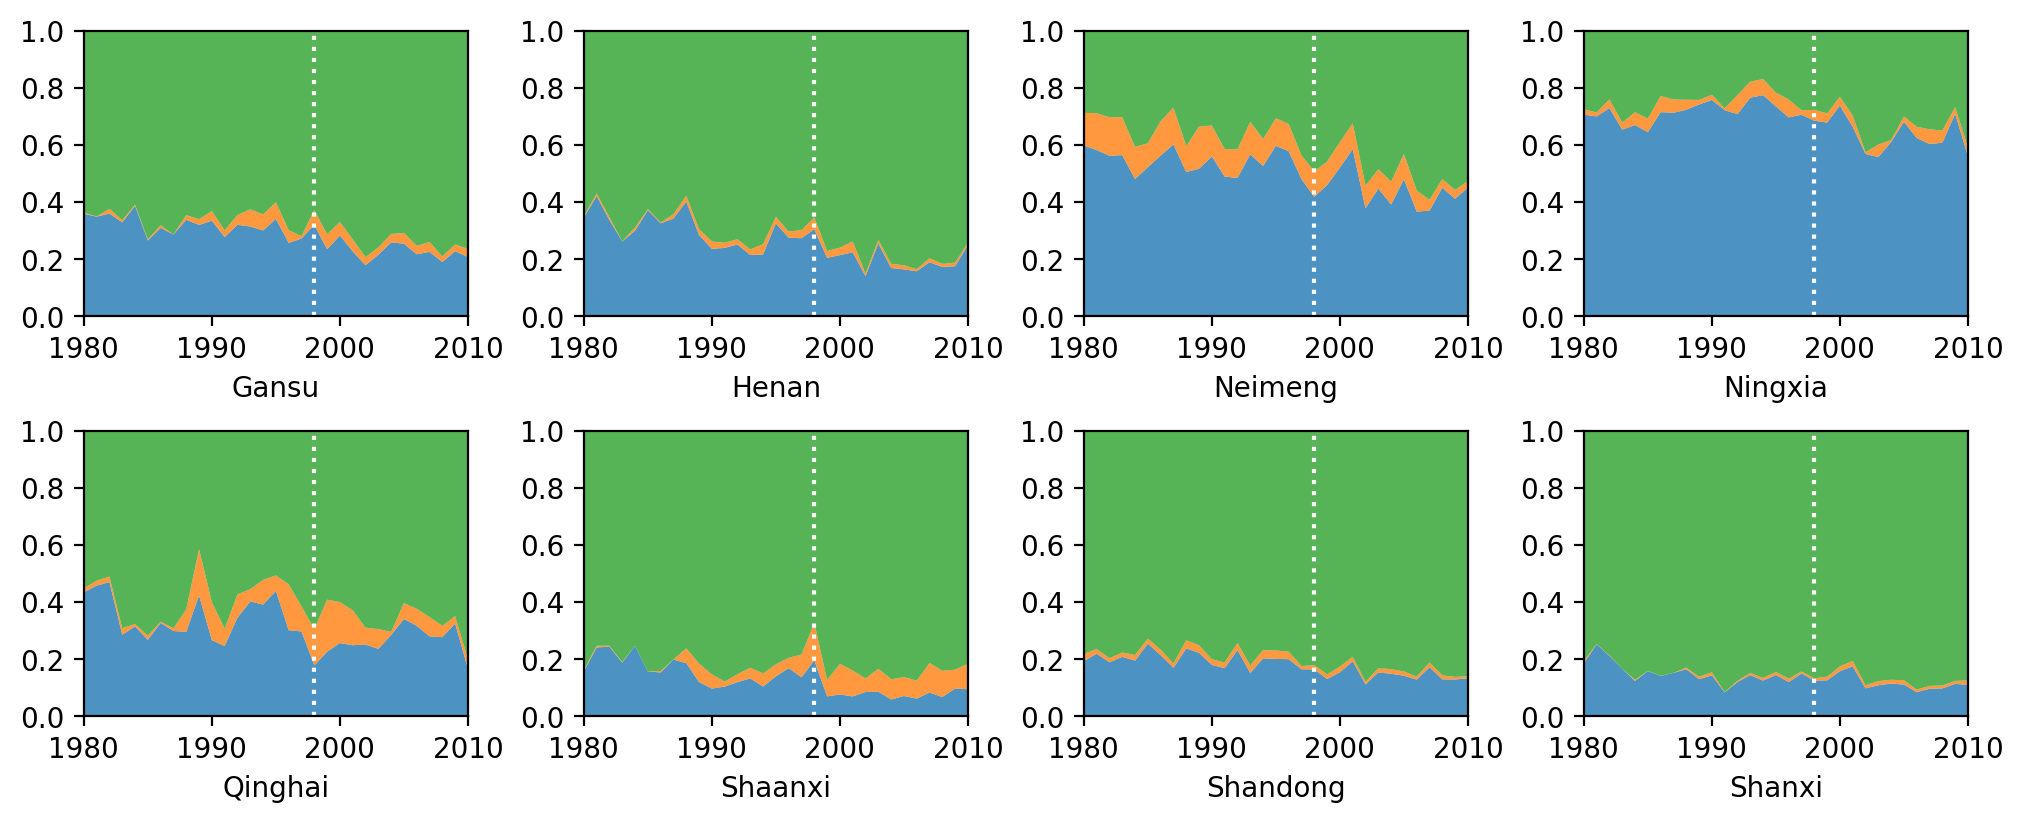
\includegraphics[width=\textwidth]{img/ch6/ch6_green_blue_water.png}
    \caption{黄河流域主要农作物用水来源的比例变化}\label{ch6:fig:sources}
\end{figure}

\subsection{地下水开采对分水制度变化的响应}

地下水使用量是分析黄河流域分水制度变化影响的重要指标。研究表明,分水制度变化对黄河流域的地下水使用量带来的影响较为明显。
具体来说,中游地区持续增加地下水的开采量,而下游地区在1987年分水制度提出之初期就开始推动节水改革。
而上游地区则先加大了地下水的开采量,在1998年统一调度制度实施后才大力推行节水改革。这些不同的反应与各地的经济发展和地下水资源的分布有关。
因此,在制定水资源管理政策和措施时,需要充分考虑不同地区的特点和实际情况,并针对性地制定相应的政策和措施。
同时,需要进一步深入研究分水制度变化对地下水使用量的影响机制,为制定更有效的水资源管理政策提供科学依据。

\begin{figure}[htb]
    \centering
    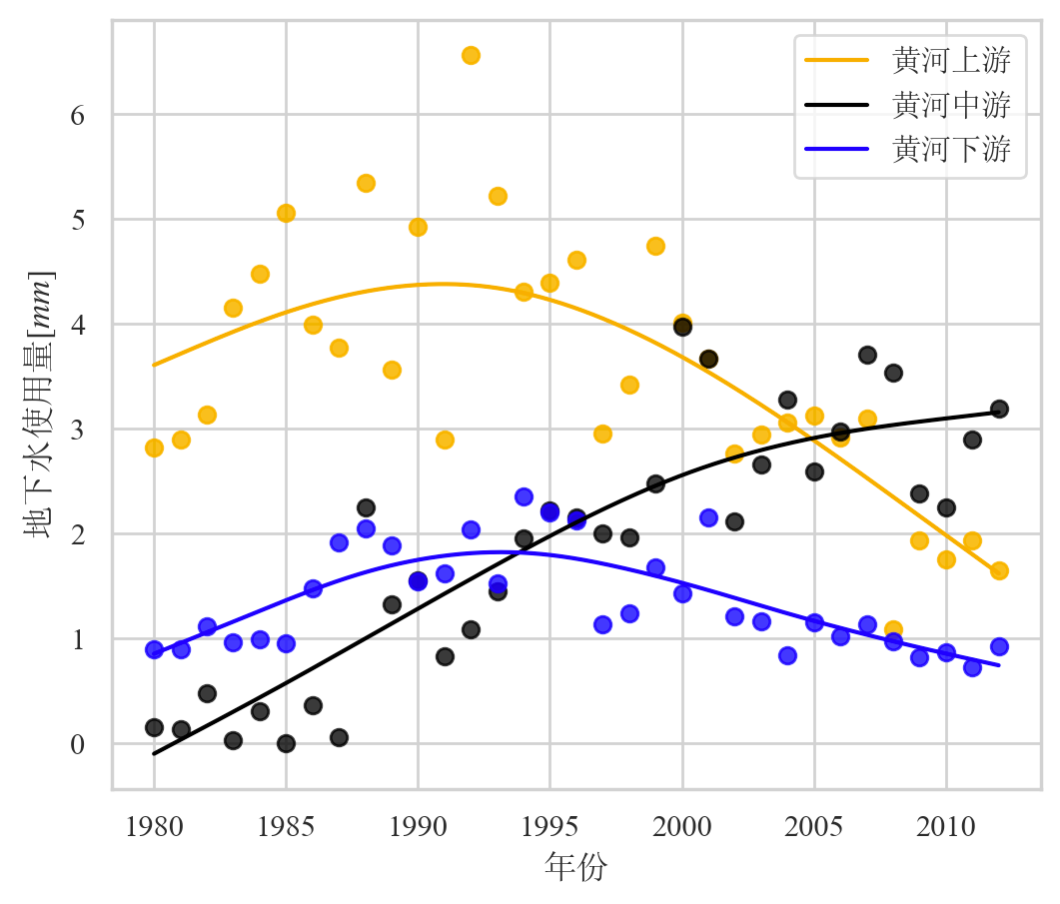
\includegraphics[width=0.6\textwidth]{img/ch6/ch6_groundwater.png}
    \caption{黄河流域、中、下游地下水开采量对分水制度变化的响应}\label{ch6:fig:groundwater}
\end{figure}